\documentclass{beamer}
\usetheme{Warsaw}
% \usepackage{beamerthemesplit} // Activate for custom appearance

\newcommand{\bbR}{\mathbb{R}}
\newcommand{\bbZ}{\mathbb{Z}}
\newcommand{\vb}{\vec{b}}
\newcommand{\vv}{\vec{v}}
\newcommand{\vvs}{\vec{v}^*}
\newcommand{\vbs}{\vec{b}^*}
\newcommand{\sspan}{\mathsf{span}}
\newcommand{\vol}{\mathrm{vol}}
\newcommand{\GH}{\mathrm{GH}}
\newcommand{\ENUMCost}{\mathrm{ENUMCost}}
\newcommand{\MINCost}{\mathrm{MINCost}}
\newcommand{\SimENUMCost}{\mathrm{Sim}\text{-}\mathrm{ENUMCost}}
\newcommand{\Costbeta}{\mathrm{Cost}_{\beta}}
\newcommand{\SimGSLengths}{\mathrm{Sim}\text{-}\mathrm{GS}\text{-}\mathrm{Lengths}}
\newcommand{\SimFEC}{\mathrm{Sim}\text{-}\mathrm{FEC}}
\newcommand{\SimGH}{\mathrm{Sim}\text{-}\mathrm{GH}}
\newcommand{\TimeBKZ}{\mathrm{TimeBKZ}}

\newtheorem*{remark}{Remark}

\title{Improved Progressive BKZ Algorithms and Their Precise Cost Estimation by Sharp Simulator}
\author{Yuncong Zhang}
\date{April 10, 2020}

\begin{document}

\frame{\titlepage}

\frame{\tableofcontents}

\section{Introduction}
\frame
{
  \frametitle{Introduction}
  The \emph{Shortest Vector Problem} (SVP):
  \begin{itemize}
  	\item Given the lattice $L=L(\vb_1,\cdots,\vb_n)$
  	\item Find the shortest non-zero vector $\vvs\in L$
  \end{itemize}
}

\frame
{
  \frametitle{Introduction}
  Current algorithms for solving SVP:
  \begin{itemize}
  	\item Blockwise: LLL, BKZ
  	\item Enumeration
  	\item Seiving
  \end{itemize}
}

\frame
{
  \frametitle{Introduction}
  Blockwise algorithms:
  \begin{itemize}
  	\item Efficiency: polynomial time for appropriate parameters
  	\item Quality: exponential approximation factor
  \end{itemize}
  Enumeration algorithms:
  \begin{itemize}
  	\item Efficiency: exponential
  	\item Quality: exact solution
  \end{itemize}
  Relationships:
  \begin{itemize}
  	\item Blockwise algorithms invokes enumeration algorithm on local blocks
  	\item Enumeration algorithm requires preprocessing by blockwise algorithms
  \end{itemize}
}

\frame
{
  \frametitle{Introduction}
  BKZ Algorithms:
  \begin{itemize}
  	\item Basic BKZ (proposed by C. P. Schnorr in 1994)
  	\item BKZ 2.0
  	\item Progressive BKZ
  \end{itemize}
}

\section{Preliminaries}
\frame{
	\frametitle{Preliminaries}
	\begin{itemize}
		\item Mathematical Definitions
		\item Enumeration Algorithm
		\item LLL Algorithm
	\end{itemize}
}

\subsection{Mathematical Definitions}
\frame{
	\frametitle{Mathematical Definitions}
	Gram-Schmidt Basis for $B=(\vb_1,\cdots,\vb_n)$:
	\begin{itemize}
		\item $B^*:=(\vb_1^*,\cdots,\vb_n^*)$
		\item $\vb_i^*:=\vb_i-\sum_{j=1}^{i-1}\mu_{ij}\cdot\vb_j^*$
		\item $\mu_{ij}:=\langle\vb_i,\vb_j^*\rangle/\|\vb_j^*\|^2$ called GS coefficients
	\end{itemize}
	Properties:
	\begin{itemize}
		\item $\vol(L):=\det(L):=\det(B)=\det(B^*)=\prod_{i=1}^n \|\vb_i^*\|$
		\item Gram-Schmidt Assumption (GSA): $\|\vb_i^*\|^2/\|\vb_1\|^2=r^{i-1}$, where $r\in[3/4,1)$ is GSA constant
	\end{itemize}
}

\frame{
	\frametitle{Mathematical Definitions}

	\begin{figure}[ht!]
	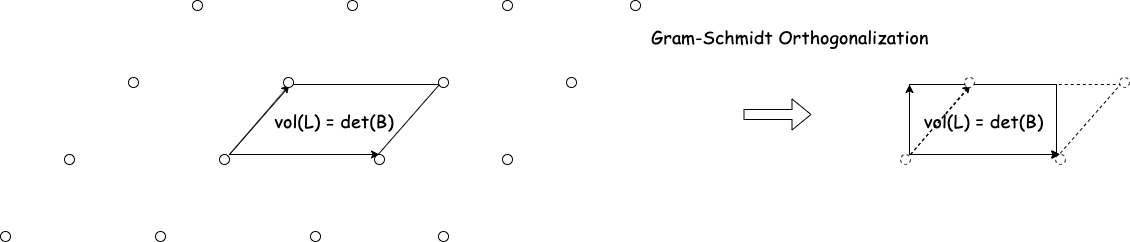
\includegraphics[width=0.8\textwidth]{files/BKZ-Volume.png}
	\caption{Gram-Schmidt orthogonalization and volume of lattice}
	\label{fig:bkz.volume}
	\end{figure}
}

\frame{
	\frametitle{Mathematical Definitions}
	Projection $\pi_i:\bbR^n\to\sspan(\vb_1,\cdots,\vb_{i-1})^{\perp}$
	\begin{eqnarray}
	\pi_i(v):=\vec{v}-\sum_{j=1}^{i-1}\langle\vec{v},\vb_j^*\rangle\vb_j^*/\|\vb_j^*\| \label{eqn:pi}
	\end{eqnarray}
	which effectively removes the proportion of the vector inside the space $\sspan(\vb_1,\cdots,\vb_{i-1})$.
	\begin{remark}
	Gram-Schmidt reduction can be rewritten as: $\vb_i^* = \pi_i(\vb_i)$
	\end{remark}
}

\frame{
	\frametitle{Mathematical Definitions}
	Projective \emph{local block}
	\begin{eqnarray}
	L_{[i:j]} &:=& \pi_i(L(\vb_i,\vb_{i+1},\cdots,\vb_j))
	\end{eqnarray}
	Use $B_i:=L_{[i:i+\beta-1]}$ when the blocksize $\beta$ is clear
}

\frame{
	\frametitle{Mathematical Definitions}

	\begin{figure}[ht!]
	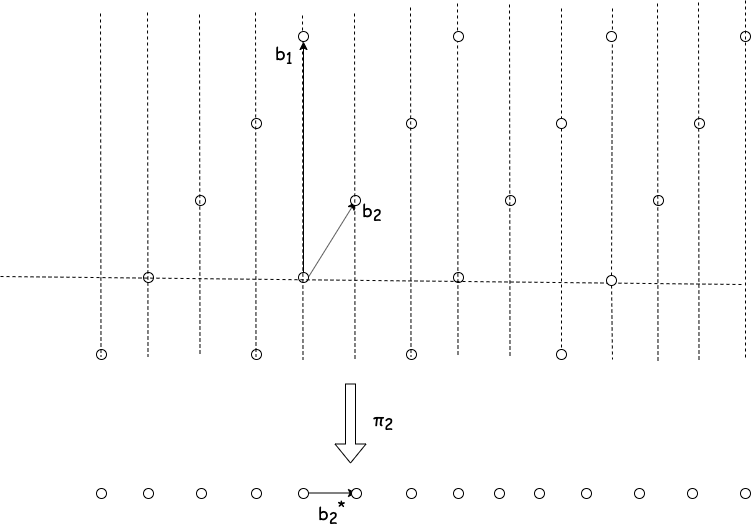
\includegraphics[width=0.7\textwidth]{files/BKZ-Projection.png}
	\caption{Projection $\pi_2$ on a lattice}
	\label{fig:proj}
	\end{figure}
}

\frame{
	\frametitle{Mathematical Definitions}
	Gaussian Huristic: for convex set $S$
	\begin{itemize}
		\item $|S\cap L|\approx\vol(S)/\vol(L)$
		\item $\GH(L):=(\vol(L)/V_n(1))^{1/n}$ approximation of $\lambda_1(L)$
	\end{itemize}

	\begin{remark}
	$V_n(R)$ is the volume of the $n$-dimensional ball.
	\[V_n(R) = R^n\cdot\frac{\pi^{n/2}}{\Gamma(n/2+1)}\]
	\end{remark}
}

\frame{
	\frametitle{Mathematical Definitions}
	Modified Gaussian heuristic for local blocks:
	\begin{itemize}
		\item For local blocks $B_i$ and small blocksize $\beta$, $\GH(B_i)$ is often smaller than $\lambda_1(L)$
		\item Approximates $\lambda_1(L)$ with $\tau_i\GH(B_i)$ instead
	\end{itemize}
	where
	\[
	\tau_i:=\frac{\|\vb_{n-i+1}^*\|}{V_i(1)^{-1/i}\cdot\prod_{j=n-i+1}^n\|\vb_j^*\|^{1/i}}
	\]
	is called modified Gaussian heuristic constant.
}

\subsection{Enumeration Algorithm}
\frame{
	\frametitle{Enumeration Algorithm}
	Given a lattice basis $B=(\vb_1,\cdots,\vb_n)$, finds the shortest vector $\vvs$
	\[
	\vvs=a_1\vb_1+a_2\vb_2+\cdots+a_n\vb_n\qquad\forall i\in[n]
	\]
	Observation:
	\begin{itemize}
		\item $\|\pi_i(a_i\vb_i+\cdots+a_n\vb_n)\|=\|\pi_i(\vvs)\|\leq\|\vvs\|\approx R_i$
		\item For $i=n$, $|a_n|\leq R_n/\|\vb_n^*\|$
		\item Fix $a_n,\cdots,a_{i+1}$, then $|a_i|$ is bounded
	\end{itemize}
}

\frame{
	\frametitle{Enumeration Algorithm}
	Searching tree:
	\begin{itemize}
		\item Root: zero vector $\vec{0}$
		\item Children of $\vv$ (at depth $k$): $\vv+a_{n-k}\vb_{n-k}\quad\forall a_{n-k}\in\bbZ$ bounded by $R_{n-k}$ projected by $\pi_{n-k+1}(\cdot)$
		\item Nodes at depth $k$: $\forall\vv\in\bbR^n$ with $\|\pi_k(\vv)\|$ bounded by $R_{n-k+1}$
	\end{itemize}
}

\frame{
	\frametitle{Enumeration Algorithm}
	\begin{figure}[ht!]
		\centering
		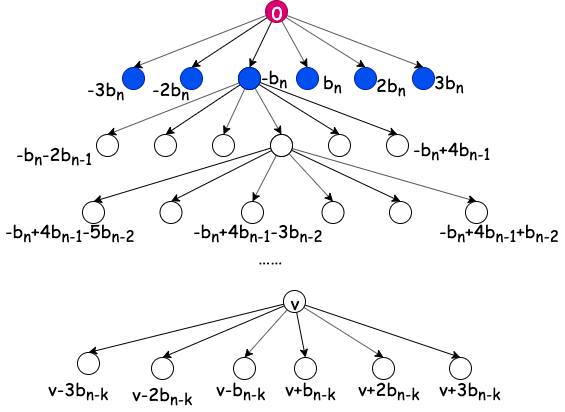
\includegraphics[width=0.6\textwidth]{files/BKZ-Searching-Tree.png}
		\caption{Searching Tree}
		\label{fig:search-tree}
	\end{figure}
}

\subsection{LLL Algorithm}
\frame{
	\frametitle{LLL Algorithm}
}


\section{Previous BKZ Algorithms}
\frame{
	\frametitle{Previous BKZ Algorithms}
}

\subsection{Basic BKZ Algorithm}
\frame{
	\frametitle{Basic BKZ Algorithm}
}

\subsection{BKZ 2.0}
\frame{
	\frametitle{BKZ 2.0}
}

\subsection{Progressive BKZ}
\frame{
	\frametitle{Progressive BKZ}
}

\section{Improved Progressive BKZ}
\frame{
	\frametitle{Improved Progressive BKZ}
}

\subsection{Optimizing Parameters}
\frame{
	\frametitle{Optimizing Parameters}
}

\subsection{Estimating Enumeration Cost}
\frame{
	\frametitle{Estimating Enumeration Cost}
}

\subsection{Blocksize Strategy}
\frame{
	\frametitle{Blocksize Strategy}
}

\subsection{BKZ Rounds}
\frame{
	\frametitle{BKZ Rounds}
}

\subsection{Pre/Post-Processing}
\frame{
	\frametitle{Pre/Post-Processing}
}

\frame{
	\center{Q/A}
}

\end{document}
